\documentclass[a4paper,11pt, a4paper]{article}


\usepackage{amsmath,amssymb}
\usepackage{graphicx}
\usepackage{epsfig}
\usepackage{dirtytalk}
\usepackage{xcolor}
\usepackage{listings}
\usepackage{charter}
\usepackage{lmodern}
\usepackage{geometry}
\usepackage[T1]{fontenc}
\lstset{
basicstyle=\ttfamily,
numbers=left,
numberstyle=\tiny,
stepnumber=1,
numbersep=5pt,
breaklines=true,
postbreak=\mbox{\textcolor{red}{\(\hookrightarrow\)}\space},
keywordstyle=\bfseries,
}
\usepackage{graphicx}
\usepackage{sidecap}

\begin{document}

\title{Outer Billiard Report}
\author{Evan Huynh}
\maketitle

\begin{abstract}
	This report gives a briefly look about our code and progress in the \say{Outer Billiard} project.
\end{abstract}

\tableofcontents
\listoffigures
%\listoftables
  
\section{Introduction}
This report gives a briefly look about our code and progress in the \say{Outer Billiard} project in Mathematica.\footnote{This program was originally written in Mathematica 11.}

\section{Method}
%According to the background theory provided, there is one easy way to determine the position of its symmetrical point over a middle point by calculating the directional vector of the initial point to the middle point, then by translating it with that directional vector, we obtain the position of the symmetrical point that we are needed to find.

As stated in the problem, the ball outside of the triangle travels a distance \(d\) to one corner, the continue with \(d\) before deflect to another corner. This problem can be solved using vector. Let assume there exists two points \(K \ (x_K, y_K)\) and \(L\ (x_L, y_L)\). The new point M which is a reflection of \(K\) over \(L\) will have the coordinate \(x_M = x_L - x_K\) , \( y_M = y_L - y_K\). In order word, by translating point \(L\) with \(\overrightarrow{LK}\), we obtained the coordinate of point \(M\). This concept can be demonstrate with a function \textbf{reflectPoint} in the appendix.

One such issue exist in this problem is to ascertain which corner of the \(\triangle ABC\) to draw the next symmetrical point. From the hypothesis, the billiard travel across the first corner, then the second, then the third, and repeat the process. Since the ball travels and marks the location before changing its direction, the number of marks determine which direction it goes when changing the direction.

To repeat the process systematically, we first let the ball travels to \(A\) then \(B\) and \(C\), consecutively. This can be solved using modularity. Let \(n\) be the marked location, including the initial location \(K \ (x_K, y_K)\). if \(n \equiv 1 \pmod 3\) the ball goes toward \(A\), or if \(n \equiv 2 \pmod 3\), it goes over \(B\). else it runs to \(C\). This strategy works as drawing \(n\) segments require at least \(n+1\) points, and since the drawing process repeats over three corner of the equilateral triangle, the modularity of 3 of marked points determines the next directions the ball moves.

\section{Result}
\begin{figure}
\centering
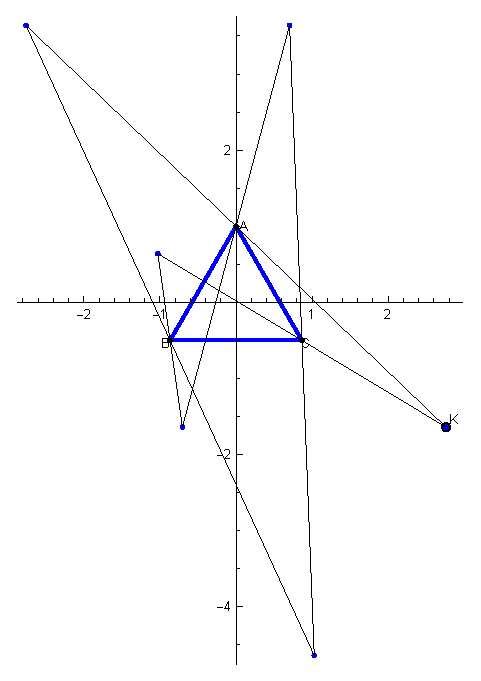
\epsfig{file=Problem_3.eps}
\caption{This figure demonstrate moving direction of the particle from outside of the triangle, generated by Mathematica.}
\end{figure}

\section{Discussion}
As shown in the figure, the point will returns to the initial position after a number of finite turns. We can prevent this from happens by randomly choosing a next corner for the next direction of the ball. Instead, we decided to keep our original solution, even though the result might not be like "Outer Billiard".

\pagebreak
\section{Appendix}
\subsection{Mathematica}
\subsubsection{Function}
\lstset{language=Mathematica}
\begin{lstlisting}
reflectPoint[outPoint_?ListQ,middlePoint_?ListQ]:=(
xMove = -(outPoint[[1]]-middlePoint[[1]]);
yMove = -(outPoint[[2]]-middlePoint[[2]]);
{middlePoint[[1]]+xMove,middlePoint[[2]]+yMove}
)
\end{lstlisting}

\subsubsection{Main program}

\lstset{language=Mathematica}
\begin{lstlisting}
Manipulate[
(*-----------------*)
(*Create the first equilateral triangle*)
triangle1=Polygon[CirclePoints[3]];
xA=0;yA=1; pointA={xA,yA}; textA= Text["A",{0.1,1}];
xB=-(Sqrt[3]/2);yB=-(1/2); pointB={xB,yB}; textB = Text ["B",{-0.92,-0.54}];
xC=Sqrt[3]/2; yC=-(1/2); pointC={xC,yC}; textC = Text["C",{0.92,-0.54}];
xK;yK; pointK={xK,yK}; textK=Text["K",{xK+0.1,yK+0.1}];
pointList={pointK};

plot2={EdgeForm[Directive[Thick,Blue]],Directive[White],triangle1,Directive[Black],Point[pointA],Point[pointB],Point[pointC],textA,textB,textC,PointSize[0.02],Point[pointK],textK};

(*Add point to list*)
doCtimes; doCtimes=Floor[doCtimes];
Do[
If[Mod[Length[pointList],3]==1,
pointList=AppendTo[pointList,reflectPoint[Last[pointList],pointA]];,
If [Mod[Length[pointList],3]==2,
pointList=AppendTo[pointList,reflectPoint[Last[pointList],pointB]];,
pointList=AppendTo[pointList,reflectPoint[Last[pointList],pointC]];
]
]
,doCtimes];
plot3={Blue,Point[pointList],Black,Line[pointList]};

(*Export the result*)
plot4={plot2,plot3};
Show[Graphics[plot4],Axes-> True,AxesStyle->Black]
(*-----------------*)

,{{xK,2,"x-coordinate"},-5,5},{{yK,2,"y-coordinate"},-5,5},{{doCtimes,3,"Number of movements"},0,10}]
\end{lstlisting}

\end{document}
